\documentclass[11pt,a4paper]{article}

\usepackage[margin=1in]{geometry}
\usepackage{mathptmx}
\usepackage{amsmath}
\usepackage{amssymb}
\usepackage{amsthm}
\usepackage{braket}
\usepackage{tikz}
\usepackage{quantikz}
\usepackage{enumitem}
\usepackage{hyperref}
\usepackage{xcolor}

\definecolor{circuitblue}{RGB}{40,80,160}

\hypersetup{
    colorlinks=true,
    linkcolor=circuitblue,
    urlcolor=circuitblue,
    citecolor=circuitblue
}

\theoremstyle{definition}
\newtheorem{definition}{Definition}[section]
\newtheorem{example}{Example}[section]

\theoremstyle{remark}
\newtheorem*{intuition}{Intuition}
\newtheorem*{keypoint}{Key Point}

\pagestyle{plain}

\setlength{\parindent}{0pt}
\setlength{\parskip}{6pt}

\begin{document}

\begin{center}
    {\LARGE \textbf{Advanced Classical ML and Variational Algorithms}}\\[8pt]
    {\large QML}\\[12pt]
    \hrule
\end{center}

\vspace{12pt}
\tableofcontents
\newpage

%% ========================================================
\section{Overview}
%% ========================================================

this lecture goes deep into the two classical ML paradigms that directly inspire QML: \textbf{kernel methods} and \textbf{neural networks}. understanding SVMs and the kernel trick is essential bcs quantum kernel methods r the most mathematically grounded approach to QML. and understanding neural networks is essential bcs variational quantum circuits (PQCs) r essentially the quantum analogue of neural networks.

by the end of this lecture, u should see exactly where quantum fits into the classical ML picture.

%% ========================================================
\section{Support Vector Machines}
%% ========================================================

\subsection{Linear SVM: The Idea}

\begin{definition}
a \textbf{support vector machine} (SVM) finds the hyperplane that separates two classes with the \textbf{maximum margin} --- the maximum distance between the hyperplane and the nearest data points from each class.
\end{definition}

the hyperplane is defined by: $w^T x + b = 0$

classification rule: $\text{sign}(w^T x + b)$

\begin{center}
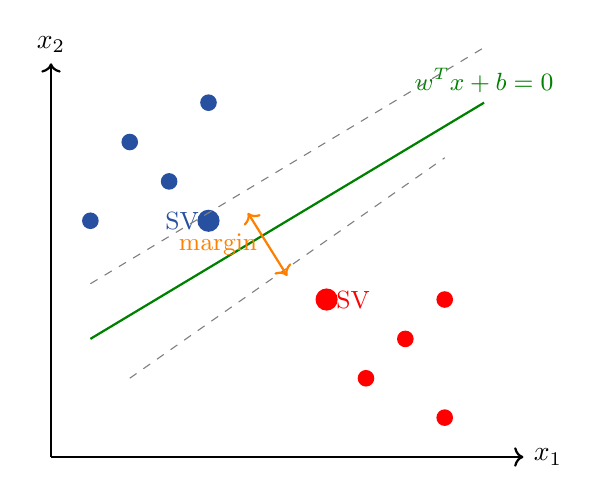
\begin{tikzpicture}[scale=1]
    \draw[->, thick] (0,0) -- (6,0) node[right] {$x_1$};
    \draw[->, thick] (0,0) -- (0,5) node[above] {$x_2$};

    % class +1
    \fill[circuitblue] (1,4) circle (3pt);
    \fill[circuitblue] (1.5,3.5) circle (3pt);
    \fill[circuitblue] (0.5,3) circle (3pt);
    \fill[circuitblue] (2,4.5) circle (3pt);
    \fill[circuitblue] (2,3) circle (4pt) node[left, font=\small] {SV};

    % class -1
    \fill[red] (4,1) circle (3pt);
    \fill[red] (4.5,1.5) circle (3pt);
    \fill[red] (5,0.5) circle (3pt);
    \fill[red] (3.5,2) circle (4pt) node[right, font=\small] {SV};
    \fill[red] (5,2) circle (3pt);

    % decision boundary
    \draw[thick, green!50!black] (0.5,1.5) -- (5.5,4.5) node[above, font=\small] {$w^T x + b = 0$};

    % margin lines
    \draw[dashed, gray] (1,1) -- (5,3.8);
    \draw[dashed, gray] (0.5,2.2) -- (5.5,5.2);

    % margin
    \draw[<->, thick, orange] (3,2.3) -- (2.5,3.1) node[midway, left, font=\small] {margin};
\end{tikzpicture}
\end{center}

the points closest to the boundary r called \textbf{support vectors} --- they ``support'' the hyperplane. only these points determine the decision boundary.

\subsection{Primal Formulation}

the optimization problem (hard margin SVM):

\[
\boxed{\min_{w, b} \frac{1}{2}\|w\|^2 \quad \text{subject to} \quad y_i(w^T x_i + b) \geq 1 \quad \forall i}
\]

the constraint says every point must be on the correct side of the margin. minimizing $\|w\|^2$ maximizes the margin (margin $= 2/\|w\|$).

\subsection{Soft Margin SVM}

real data is rarely perfectly separable. the \textbf{soft margin SVM} allows some misclassifications by introducing slack variables $\xi_i \geq 0$:

\[
\min_{w, b, \xi} \frac{1}{2}\|w\|^2 + C\sum_{i=1}^N \xi_i \quad \text{subject to} \quad y_i(w^T x_i + b) \geq 1 - \xi_i, \quad \xi_i \geq 0
\]

$C > 0$ is the regularization parameter:
\begin{itemize}
    \item large $C$: penalize misclassifications heavily (closer to hard margin)
    \item small $C$: allow more misclassifications (smoother boundary, better generalization)
\end{itemize}

\subsection{Dual Formulation}

using lagrange multipliers $\alpha_i \geq 0$ for each constraint, the dual problem is:

\[
\boxed{\max_\alpha \sum_{i=1}^N \alpha_i - \frac{1}{2}\sum_{i,j=1}^N \alpha_i \alpha_j y_i y_j (x_i^T x_j) \quad \text{s.t.} \quad \sum_i \alpha_i y_i = 0, \quad 0 \leq \alpha_i \leq C}
\]

\begin{keypoint}
the key observation: the dual formulation only depends on the data through \textbf{inner products} $x_i^T x_j$. the decision function is:
\[
f(x) = \text{sign}\left(\sum_{i \in \text{SVs}} \alpha_i y_i (x_i^T x) + b\right)
\]
this opens the door to the \textbf{kernel trick}: replace $x_i^T x_j$ with $K(x_i, x_j) = \phi(x_i)^T \phi(x_j)$ for some feature map $\phi$ --- without ever computing $\phi$ explicitly.
\end{keypoint}

%% ========================================================
\section{The Kernel Trick}
%% ========================================================

\subsection{Feature Maps}

the problem with linear SVMs: many real-world datasets r not linearly separable. the solution: map the data to a higher-dimensional space where it \textbf{is} linearly separable.

\begin{definition}
a \textbf{feature map} $\phi: \mathcal{X} \to \mathcal{F}$ maps input data to a (possibly infinite-dimensional) feature space $\mathcal{F}$. the SVM is applied in $\mathcal{F}$ where the data may be linearly separable.
\end{definition}

\begin{example}
data in $\mathbb{R}^2$: $x = (x_1, x_2)$.

feature map: $\phi(x) = (x_1^2, \sqrt{2}x_1 x_2, x_2^2) \in \mathbb{R}^3$.

a circle in the original space becomes a hyperplane in feature space.
\end{example}

\subsection{The Kernel Function}

\begin{definition}
a \textbf{kernel function} $K: \mathcal{X} \times \mathcal{X} \to \mathbb{R}$ computes the inner product in feature space without explicitly computing the feature map:
\[
\boxed{K(x, x') = \langle \phi(x), \phi(x') \rangle_{\mathcal{F}}}
\]
\end{definition}

\begin{keypoint}
the \textbf{kernel trick}: replace every inner product $\langle x_i, x_j \rangle$ in the SVM dual with $K(x_i, x_j)$. this implicitly works in the high-dimensional feature space $\mathcal{F}$ without ever computing $\phi(x)$ explicitly.

dual SVM with kernels:
\[
\max_\alpha \sum_i \alpha_i - \frac{1}{2}\sum_{i,j} \alpha_i \alpha_j y_i y_j K(x_i, x_j)
\]

decision function:
\[
f(x) = \text{sign}\left(\sum_{i \in \text{SVs}} \alpha_i y_i K(x_i, x) + b\right)
\]
\end{keypoint}

\subsection{Common Kernels}

\textbf{linear kernel}:
\[
K(x, x') = x^T x'
\]
feature space = input space. no nonlinearity.

\textbf{polynomial kernel}:
\[
K(x, x') = (x^T x' + c)^d
\]
feature space contains all monomials up to degree $d$.

\begin{example}
for $d = 2$, $c = 0$, $x \in \mathbb{R}^2$:
\[
K(x, x') = (x_1 x_1' + x_2 x_2')^2 = x_1^2 {x_1'}^2 + 2x_1 x_2 x_1' x_2' + x_2^2 {x_2'}^2
\]
this corresponds to $\phi(x) = (x_1^2, \sqrt{2}x_1 x_2, x_2^2)$ --- the quadratic feature map.
\end{example}

\textbf{radial basis function (RBF) / gaussian kernel}:
\[
\boxed{K(x, x') = \exp\left(-\frac{\|x - x'\|^2}{2\sigma^2}\right)}
\]

\begin{intuition}
the RBF kernel is special bcs its feature space is \textbf{infinite-dimensional}. u can show that the corresponding feature map $\phi$ maps data into an infinite-dimensional hilbert space. the kernel trick lets u work in this infinite space implicitly --- u only ever compute the kernel function, which is cheap.

this is directly analogous to quantum kernels: the quantum feature map $\phi(x) = U(x)\ket{0}$ maps data into the $2^n$-dimensional hilbert space of $n$ qubits. computing the kernel $K(x, x') = |\braket{\phi(x')|\phi(x)}|^2$ on a quantum computer is efficient, even tho the feature space is exponentially large.
\end{intuition}

\subsection{Mercer's Theorem}

\begin{definition}
\textbf{Mercer's theorem}: a function $K: \mathcal{X} \times \mathcal{X} \to \mathbb{R}$ is a valid kernel (i.e., corresponds to some feature map and inner product) if and only if the \textbf{kernel matrix} (Gram matrix) $K_{ij} = K(x_i, x_j)$ is \textbf{positive semidefinite} for any set of data points $\{x_1, \ldots, x_N\}$.
\end{definition}

this is important: any positive semidefinite function can be used as a kernel. u dont need to find the feature map explicitly --- u just need to verify the PSD property.

\begin{keypoint}
quantum kernels r valid kernels bcs:
\[
K(x, x') = |\braket{\phi(x')|\phi(x)}|^2 = \text{tr}(\rho(x)\rho(x'))
\]
where $\rho(x) = \ket{\phi(x)}\bra{\phi(x)}$. the kernel matrix $K_{ij} = \text{tr}(\rho(x_i)\rho(x_j))$ is always PSD bcs its a gram matrix of density operators under the hilbert-schmidt inner product.
\end{keypoint}

%% ========================================================
\section{Neural Networks}
%% ========================================================

\subsection{The Perceptron}

\begin{definition}
a \textbf{perceptron} is the simplest neural network unit:
\[
f(x) = \sigma(w^T x + b)
\]
where $\sigma$ is a nonlinear activation function.
\end{definition}

a single perceptron can only learn linearly separable functions (same as a linear SVM). to handle nonlinear problems, u need to \textbf{stack layers}.

\subsection{Multi-Layer Perceptron (MLP)}

\begin{definition}
an \textbf{MLP} (fully connected feedforward neural network) with $L$ layers:
\[
f(x) = \sigma_L(W_L \cdot \sigma_{L-1}(W_{L-1} \cdots \sigma_1(W_1 x + b_1) \cdots + b_{L-1}) + b_L)
\]
each layer applies: linear transformation $\to$ nonlinear activation.
\end{definition}

\begin{center}
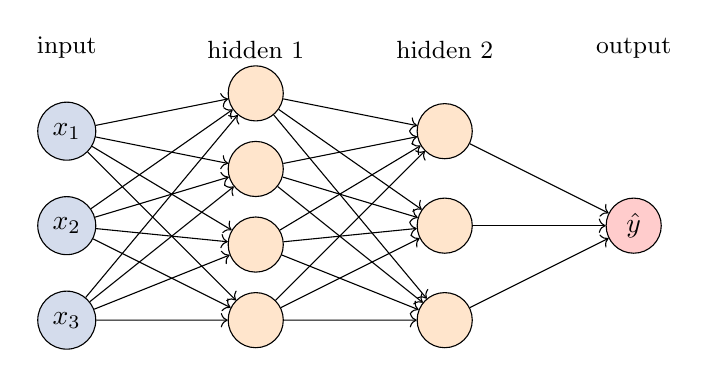
\begin{tikzpicture}[scale=0.8]
    % input layer
    \foreach \i in {1,2,3} {
        \node[draw, circle, minimum size=0.7cm, fill=circuitblue!20] (i\i) at (0, -\i*1.5+3) {$x_\i$};
    }

    % hidden layer 1
    \foreach \j in {1,2,3,4} {
        \node[draw, circle, minimum size=0.7cm, fill=orange!20] (h\j) at (3, -\j*1.2+3.3) {};
    }

    % hidden layer 2
    \foreach \k in {1,2,3} {
        \node[draw, circle, minimum size=0.7cm, fill=orange!20] (g\k) at (6, -\k*1.5+3) {};
    }

    % output layer
    \node[draw, circle, minimum size=0.7cm, fill=red!20] (o1) at (9, 0) {$\hat{y}$};

    % connections
    \foreach \i in {1,2,3} {
        \foreach \j in {1,2,3,4} {
            \draw[->] (i\i) -- (h\j);
        }
    }
    \foreach \j in {1,2,3,4} {
        \foreach \k in {1,2,3} {
            \draw[->] (h\j) -- (g\k);
        }
    }
    \foreach \k in {1,2,3} {
        \draw[->] (g\k) -- (o1);
    }

    % labels
    \node[above, font=\small] at (0, 2.5) {input};
    \node[above, font=\small] at (3, 2.5) {hidden 1};
    \node[above, font=\small] at (6, 2.5) {hidden 2};
    \node[above, font=\small] at (9, 2.5) {output};
\end{tikzpicture}
\end{center}

\subsection{Activation Functions}

\textbf{sigmoid}: $\sigma(z) = \frac{1}{1 + e^{-z}}$ --- squashes to $[0, 1]$. used for output probabilities. suffers from vanishing gradients.

\textbf{tanh}: $\sigma(z) = \tanh(z) = \frac{e^z - e^{-z}}{e^z + e^{-z}}$ --- squashes to $[-1, 1]$. zero-centered. also vanishing gradients.

\textbf{ReLU}: $\sigma(z) = \max(0, z)$ --- the workhorse of modern deep learning. simple, doesnt saturate for positive inputs. can have ``dead neurons'' ($z < 0$ always).

\textbf{softmax} (for multi-class output): $\sigma(z_i) = \frac{e^{z_i}}{\sum_j e^{z_j}}$ --- converts a vector of scores into probabilities.

\begin{intuition}
in quantum circuits, the ``activation function'' is implicit in the measurement process. the born rule ($p = |\braket{y|\psi}|^2$) is inherently nonlinear. so a quantum circuit followed by measurement is analogous to a neural network layer with a specific activation function. the key difference: quantum circuits operate with \textbf{unitary} transformations (norm-preserving), while neural networks use arbitrary linear maps + pointwise nonlinearities.
\end{intuition}

\subsection{Backpropagation}

\begin{definition}
\textbf{backpropagation} (backprop) is the algorithm for computing gradients of the loss with respect to all parameters in a neural network, using the chain rule:
\[
\frac{\partial \mathcal{L}}{\partial W_l} = \frac{\partial \mathcal{L}}{\partial a_L} \cdot \frac{\partial a_L}{\partial a_{L-1}} \cdots \frac{\partial a_{l+1}}{\partial a_l} \cdot \frac{\partial a_l}{\partial W_l}
\]
where $a_l$ is the activation of layer $l$.
\end{definition}

backprop computes all gradients in $O(d)$ time (where $d$ is the number of parameters), which is the same cost as one forward pass. this is why neural networks r trainable --- computing gradients is cheap.

\begin{keypoint}
backprop vs parameter shift rule:
\begin{itemize}
    \item \textbf{classical backprop}: compute all $p$ gradients with 1 forward + 1 backward pass. cost: $O(1) \times$ forward pass.
    \item \textbf{quantum parameter shift}: each gradient requires 2 circuit evaluations. cost: $O(p) \times$ circuit evaluation for all $p$ gradients.
    \item this $O(p)$ overhead is one of the practical bottlenecks of variational quantum algorithms. various tricks (simultaneous perturbation, adjoint methods, etc.) try to reduce it.
\end{itemize}
\end{keypoint}

\subsection{Universal Approximation Theorem}

\begin{definition}
the \textbf{universal approximation theorem} (Cybenko 1989, Hornik 1991): a neural network with a single hidden layer and sufficiently many neurons can approximate any continuous function on a compact subset of $\mathbb{R}^n$ to arbitrary accuracy.
\end{definition}

this is an existence result --- it says the approximation EXISTS but says nothing abt how to FIND it (optimization is hard). also, the required number of neurons may be exponentially large.

\begin{keypoint}
quantum analogue: perez-salinas et al. (2020) showed that data re-uploading (encoding classical data multiple times into a single qubit) makes even a single-qubit circuit a universal function approximator. the quantum version of the universal approximation theorem is: sufficiently deep PQCs with data re-uploading can approximate any function. but again, ``sufficiently deep'' may be impractically deep, and trainability (barren plateaus) is a concern.
\end{keypoint}

%% ========================================================
\section{Connection Between Kernels and Neural Networks}
%% ========================================================

\subsection{Neural Tangent Kernel}

\begin{definition}
the \textbf{neural tangent kernel} (NTK) connects neural networks to kernel methods. for a neural network $f_\theta(x)$ with parameters $\theta$, the NTK is:
\[
K_{\text{NTK}}(x, x') = \left\langle \frac{\partial f_\theta}{\partial \theta}, \frac{\partial f_\theta}{\partial \theta'} \right\rangle = \sum_i \frac{\partial f_\theta(x)}{\partial \theta_i} \frac{\partial f_\theta(x')}{\partial \theta_i}
\]
\end{definition}

in the infinite-width limit, the NTK becomes deterministic and constant during training. the neural network is equivalent to kernel regression with the NTK. this bridges the two paradigms.

\begin{intuition}
why does this matter for QML? bcs the same analysis applies to quantum circuits:

\begin{itemize}
    \item a variational quantum circuit $f_\theta(x) = \text{tr}(O \cdot U(\theta, x)\rho U^\dagger(\theta, x))$ defines a function of the data and parameters
    \item the ``quantum NTK'' is $K_{\text{QNTK}}(x, x') = \sum_i \frac{\partial f}{\partial \theta_i}(x) \frac{\partial f}{\partial \theta_i}(x')$
    \item schuld (2021) showed that variational quantum models r mathematically equivalent to kernel methods: every variational model implicitly defines a kernel, and the training dynamics can be understood through this kernel
    \item this unification is one of the deepest results in QML theory
\end{itemize}
\end{intuition}

\subsection{The Two Paradigms of QML}

\begin{keypoint}
the kernel-NN duality in QML:
\begin{center}
\begin{tabular}{l|l}
\textbf{quantum kernel methods} & \textbf{variational quantum models} \\
\hline
fix the feature map $\phi(x) = U(x)\ket{0}$ & train the circuit $U(\theta, x)$ \\
compute kernel $K(x_i, x_j)$ on quantum hardware & optimize $\theta$ on classical computer \\
train SVM/regression classically & end-to-end training \\
no barren plateaus (no parameter optimization) & barren plateaus possible \\
inductive bias fixed by circuit design & inductive bias learned during training \\
well-understood mathematically & harder to analyze theoretically \\
need quantum computer only for kernel computation & need quantum computer in the training loop
\end{tabular}
\end{center}
these two approaches r the main paradigms of QML. lectures 9--14 explore both in depth.
\end{keypoint}

%% ========================================================
\section{Deep Learning Architectures (Brief)}
%% ========================================================

\subsection{Convolutional Neural Networks (CNNs)}

CNNs exploit spatial structure using:
\begin{itemize}
    \item \textbf{convolutional layers}: apply learnable filters that slide over the input, detecting local patterns
    \item \textbf{pooling layers}: downsample spatial dimensions
    \item \textbf{parameter sharing}: the same filter is applied at every position, reducing parameter count
\end{itemize}

quantum analogue: \textbf{quantum convolutional neural networks} (QCNNs) --- circuits with local gates applied in a translational-invariant pattern, followed by measurement-based pooling (tracing out qubits). qcnns r one of the few QML architectures that provably avoid barren plateaus (Pesah et al. 2021).

\subsection{Recurrent Neural Networks (RNNs)}

RNNs process sequential data by maintaining a hidden state:
\[
h_t = \sigma(W_h h_{t-1} + W_x x_t + b)
\]

LSTM (Long Short-Term Memory) and GRU (Gated Recurrent Unit) r improved versions that handle long-range dependencies.

quantum analogue: less explored. some proposals for quantum RNNs using sequential quantum circuits, but its an open research area.

\subsection{Transformers and Attention}

the dominant architecture in modern ML (GPT, BERT, etc.). key mechanism: \textbf{self-attention}:
\[
\text{Attention}(Q, K, V) = \text{softmax}\left(\frac{QK^T}{\sqrt{d_k}}\right)V
\]

quantum analogues of attention r being explored but r very early stage. the quadratic cost of attention ($O(n^2)$ for sequence length $n$) has motivated quantum speedup proposals, but practical implementations r far off.

%% ========================================================
\section{The Variational Principle}
%% ========================================================

this section bridges classical ML optimization with quantum variational algorithms.

\begin{definition}
the \textbf{variational principle} in quantum computing: given a parameterized quantum circuit $U(\theta)$ and a cost function $C(\theta) = \langle \psi(\theta) | H | \psi(\theta) \rangle$, find the parameters $\theta^*$ that minimize $C$:
\[
\theta^* = \arg\min_\theta C(\theta) = \arg\min_\theta \text{tr}(H \cdot U(\theta)\rho_0 U^\dagger(\theta))
\]
\end{definition}

\begin{center}
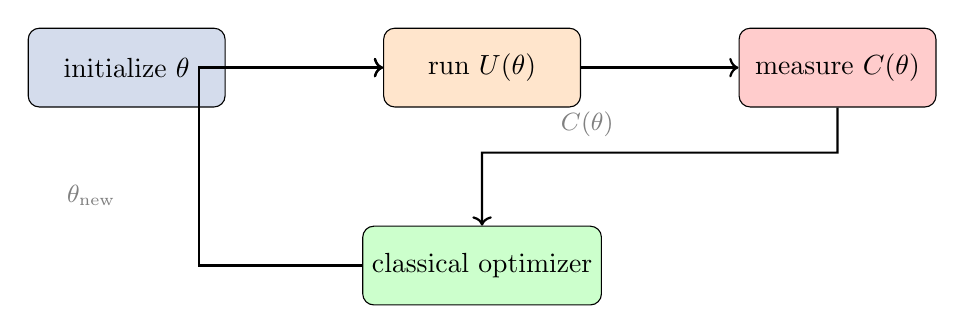
\begin{tikzpicture}[scale=0.9, node distance=2cm]
    \node[draw, rounded corners, fill=circuitblue!20, minimum width=2.5cm, minimum height=1cm] (init) {initialize $\theta$};
    \node[draw, rounded corners, fill=orange!20, minimum width=2.5cm, minimum height=1cm, right=of init] (qc) {run $U(\theta)$};
    \node[draw, rounded corners, fill=red!20, minimum width=2.5cm, minimum height=1cm, right=of qc] (meas) {measure $C(\theta)$};
    \node[draw, rounded corners, fill=green!20, minimum width=2.5cm, minimum height=1cm, below=1.5cm of qc] (opt) {classical optimizer};

    \draw[->, thick] (init) -- (qc);
    \draw[->, thick] (qc) -- (meas);
    \draw[->, thick] (meas) -- ++(0,-1.2) -| (opt);
    \draw[->, thick] (opt) -- ++(-4,0) |- (qc);

    \node[font=\small, gray] at (6.5,-0.8) {$C(\theta)$};
    \node[font=\small, gray] at (-0.5,-1.8) {$\theta_{\text{new}}$};
\end{tikzpicture}
\end{center}

a typical variational circuit for VQE looks like this:

\begin{center}
\begin{quantikz}
\lstick{$\ket{0}$} & \gate{R_Y(\theta_1)} & \ctrl{1} & \qw & \gate{R_Y(\theta_4)} & \ctrl{1} & \qw & \meter{} \\
\lstick{$\ket{0}$} & \gate{R_Y(\theta_2)} & \targ{} & \ctrl{1} & \gate{R_Y(\theta_5)} & \targ{} & \ctrl{1} & \meter{} \\
\lstick{$\ket{0}$} & \gate{R_Y(\theta_3)} & \qw & \targ{} & \gate{R_Y(\theta_6)} & \qw & \targ{} & \meter{}
\end{quantikz}
\end{center}

the parameters $\theta_1, \ldots, \theta_6$ r optimized by the classical optimizer to minimize the cost function. the circuit structure (which gates, which connectivity) is the ansatz --- its the ``architecture'' of the quantum model.

this ``quantum-classical loop'' is the standard architecture for all variational quantum algorithms:
\begin{itemize}
    \item \textbf{VQE} (variational quantum eigensolver): $C = \langle H \rangle$ for finding ground state energies
    \item \textbf{QAOA}: $C$ encodes combinatorial optimization objectives
    \item \textbf{variational quantum classifiers}: $C$ is a classification loss
    \item \textbf{quantum kernel training}: $C$ is a kernel alignment objective
\end{itemize}

\begin{keypoint}
the variational approach is the dominant paradigm for NISQ quantum computing bcs:
\begin{enumerate}
    \item circuits can be kept shallow (noise-friendly)
    \item the classical optimizer handles the hard optimization work
    \item the quantum computer only needs to estimate expectation values (not do complex coherent computation)
    \item its flexible --- same framework works for chemistry, optimization, and ML
\end{enumerate}
the main challenges: barren plateaus (flat loss landscapes), local minima, noise in gradient estimates, and the $O(p)$ cost of gradient computation via parameter shift.
\end{keypoint}

%% ========================================================
\section{Summary}
%% ========================================================

\begin{keypoint}
the big connections:
\begin{enumerate}
    \item \textbf{SVMs and kernel methods}: data is classified by inner products in a feature space. the kernel trick avoids computing the feature map. quantum kernel methods use quantum circuits as feature maps and estimate kernels on quantum hardware.
    \item \textbf{neural networks}: parameterized function approximators trained by gradient descent (backprop). variational quantum circuits r the quantum analogue --- parameterized unitaries trained by the parameter shift rule.
    \item \textbf{kernel-NN duality}: neural networks in the infinite-width limit r equivalent to kernel methods (NTK). similarly, variational quantum models r equivalent to quantum kernel methods (schuld 2021).
    \item \textbf{the variational principle}: the quantum-classical optimization loop. parameterize a quantum circuit, measure a cost function, optimize classically. this is the framework for all NISQ QML algorithms.
\end{enumerate}
\end{keypoint}

a quantum kernel circuit computes similarity between encoded data points:

\begin{center}
\begin{quantikz}
\lstick{$\ket{0}$} & \gate[2]{U_\phi(x)} & \gate[2]{U_\phi^\dagger(x')} & \meter{} \\
\lstick{$\ket{0}$} & & & \meter{}
\end{quantikz}
\end{center}

$P(\text{all zeros}) = |\braket{\phi(x')|\phi(x)}|^2 = K_Q(x, x')$. this is the quantum kernel --- well develop it fully in lectures 12--14.

with the classical ML foundation complete, were ready to dive into quantum ML properly. next: parameterized quantum circuits --- the building blocks of variational QML.

\end{document}
